% Preamble: packages, theme, and shared macros for the pipeline physics deck
\documentclass[aspectratio=169,10pt]{beamer}

\usetheme{metropolis}
\usepackage{amsmath,amssymb}
\usepackage{booktabs}
\usepackage{graphicx}
\usepackage{tikz}
\usetikzlibrary{arrows.meta,positioning,calc}
\usepackage{bm}
\usepackage[normalem]{ulem}
\usepackage{appendixnumberbeamer}

% Colours
\definecolor{cDM}{HTML}{8B0000}
\definecolor{cHI}{HTML}{006400}
\definecolor{cAstro}{HTML}{00008B}
\definecolor{cNoise}{HTML}{555555}

% Shortcuts -- observables
\newcommand{\Cl}{C_\ell}
\newcommand{\Nell}{N_\ell}
\newcommand{\Well}{W_\ell}
\newcommand{\Bell}{B_\ell}
\newcommand{\Plin}{P_{\mathrm{lin}}}
\newcommand{\sigv}{\langle\sigma v\rangle}

% Shortcuts -- cosmology
\newcommand{\OmM}{\Omega_{\mathrm{M}}}
\newcommand{\OmB}{\Omega_{\mathrm{B}}}
\newcommand{\OmDM}{\Omega_{\mathrm{DM}}}
\newcommand{\OmL}{\Omega_\Lambda}
\newcommand{\OmHI}{\Omega_{\mathrm{HI}}}
\newcommand{\rhoc}{\rho_{\mathrm{c}}}
\newcommand{\rhobar}{\bar\rho}
\newcommand{\Rvir}{R_{\mathrm{vir}}}
\newcommand{\Dvir}{\Delta_{\mathrm{vir}}}
\newcommand{\deltac}{\delta_{\mathrm{c}}}
\newcommand{\Msun}{M_\odot}
\newcommand{\Mpch}{\,\mathrm{Mpc}/h}

% Shortcuts -- HI
\newcommand{\MHI}{M_{\mathrm{HI}}}
\newcommand{\Tbar}{\bar{T}_b}
\newcommand{\bHI}{b_{\mathrm{HI}}}
\newcommand{\WHI}{W_{\mathrm{HI}}}
\newcommand{\PHI}{P_{\mathrm{HI}}}

% Shortcuts -- DM
\newcommand{\mchi}{m_\chi}
\newcommand{\WDM}{W_\gamma^{\mathrm{DM}}}
\newcommand{\Deltasq}{\Delta^2}

% Shortcuts -- astro
\newcommand{\Wastro}{W_\gamma^{\mathrm{astro}}}
\newcommand{\Lsens}{L_{\mathrm{sens}}}
\newcommand{\Fsens}{F_{\mathrm{sens}}}

% Shortcuts -- units
\newcommand{\cmtwo}{\,\mathrm{cm}^{-2}\,\mathrm{s}^{-1}}
\newcommand{\ergpers}{\,\mathrm{erg\,s}^{-1}}
\newcommand{\mK}{\,\mathrm{mK}}
\newcommand{\GeV}{\,\mathrm{GeV}}
\newcommand{\sr}{\,\mathrm{sr}}

\setbeamertemplate{footline}[frame number]

\title{HI $\times$ UGRB Cross-Correlation Pipeline}
\subtitle{Complete Physics Reference}
\author{Research Progress Update}
\date{\today}

\begin{document}

\maketitle

\begin{frame}{Outline}
\tableofcontents
\end{frame}

\section{Pipeline Overview}

\begin{frame}{Scientific Goal}
\begin{itemize}
    \item Cross-correlate \textbf{HI 21-cm intensity maps} (MeerKAT/SKA) with the \textbf{unresolved gamma-ray background} (Fermi-LAT)
    \item Detect astrophysical cross-signal (blazars, mAGN, SFGs sharing LSS with HI)
    \item Constrain dark matter annihilation via excess $\Cl^{\mathrm{HI}\times\gamma}$
    \item Based on Pinetti, Camera, Fornengo \& Regis (2020, JCAP 07:044)
\end{itemize}
\end{frame}

\begin{frame}{Module Dependency DAG}
\centering
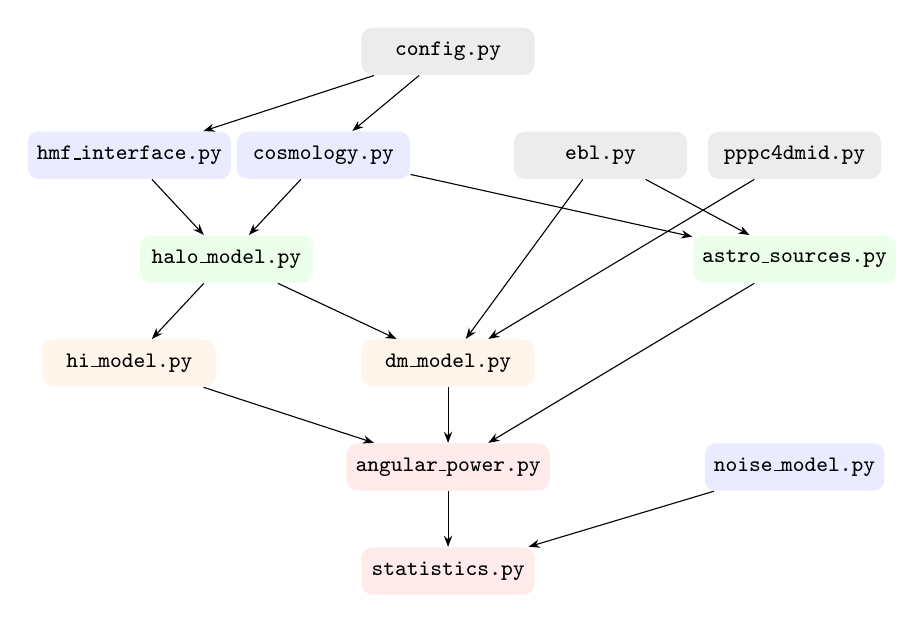
\begin{tikzpicture}[scale=0.88, every node/.append style={transform shape},
    every node/.style={font=\footnotesize, rounded corners, minimum width=2.2cm, minimum height=0.6cm, align=center},
    tier0/.style={fill=gray!15},
    tier1/.style={fill=blue!8},
    tier2/.style={fill=green!8},
    tier3/.style={fill=orange!8},
    tier4/.style={fill=red!8},
    arr/.style={-{Stealth[length=4pt]}, thin}
]
% Row 0 — top-level config
\node[tier0] (cfg) at (0, 0) {\texttt{config.py}};

% Row 1 — backbone (left) and standalone data inputs (right)
\node[tier1] (hmfi)  at (-4.6, -1.5) {\texttt{hmf\_interface.py}};
\node[tier1] (cosmo) at (-1.8, -1.5) {\texttt{cosmology.py}};
\node[tier0] (ebl)   at ( 2.2, -1.5) {\texttt{ebl.py}};
\node[tier0] (pppc)  at ( 5.0, -1.5) {\texttt{pppc4dmid.py}};

% Row 2 — intermediate physics
\node[tier2] (halo)  at (-3.2, -3.0) {\texttt{halo\_model.py}};
\node[tier2] (astro) at ( 5.0, -3.0) {\texttt{astro\_sources.py}};

% Row 3 — HI (left) and DM (centre, draws from both sides)
\node[tier3] (hi) at (-4.6, -4.5) {\texttt{hi\_model.py}};
\node[tier3] (dm) at ( 0.0, -4.5) {\texttt{dm\_model.py}};

% Row 4 — integration layer
\node[tier4] (ang)   at ( 0.0, -6.0) {\texttt{angular\_power.py}};
\node[tier1] (noise) at ( 5.0, -6.0) {\texttt{noise\_model.py}};

% Row 5 — output
\node[tier4] (stat) at (0.0, -7.5) {\texttt{statistics.py}};

% Arrows — all flow downward with no crossings
\draw[arr] (cfg)   -- (hmfi);
\draw[arr] (cfg)   -- (cosmo);
\draw[arr] (hmfi)  -- (halo);
\draw[arr] (cosmo) -- (halo);
\draw[arr] (cosmo) -- (astro);
\draw[arr] (ebl)   -- (astro);
\draw[arr] (ebl)   -- (dm);
\draw[arr] (pppc)  -- (dm);
\draw[arr] (halo)  -- (hi);
\draw[arr] (halo)  -- (dm);
\draw[arr] (hi)    -- (ang);
\draw[arr] (dm)    -- (ang);
\draw[arr] (astro) -- (ang);
\draw[arr] (ang)   -- (stat);
\draw[arr] (noise) -- (stat);
\end{tikzpicture}
\end{frame}

\begin{frame}{Unit Conventions}
\begin{table}
\centering\footnotesize
\begin{tabular}{lll}
\toprule
Quantity & Unit & Convention \\
\midrule
Distances & $\Mpch$ (comoving) & $\chi$, $\Rvir$, $r_s$ \\
Masses & $\Msun/h$ & $M$, $\MHI$ \\
Wavenumbers & $h/\mathrm{Mpc}$ & $k$ \\
Power spectra & $(\Mpch)^3$ & $\Plin$, $\PHI$ \\
Mass function & $(\Mpch)^{-3}\,(\Msun/h)^{-1}$ & $dn/dM$ \\
\midrule
Brightness temp. & mK & $\Tbar$ \\
Luminosities & erg/s & GLFs \\
Fermi noise & $\mathrm{cm}^{-4}\,\mathrm{s}^{-2}\,\mathrm{sr}^{-1}$ & $N^\gamma$ \\
\bottomrule
\end{tabular}
\end{table}
\vspace{0.3cm}
All internal calculations use $h$-dependent comoving units.\\
Physical units appear only at module boundaries (explicit conversion).
\end{frame}

\section{Cosmology}

\begin{frame}{Planck 2018 Parameters}
\begin{columns}[T]
\column{0.5\textwidth}
\begin{align*}
H_0 &= 67.36\;\mathrm{km/s/Mpc} \\
h &= 0.6736 \\
\OmB h^2 &= 0.02237 \\
\Omega_c h^2 &= 0.1200 \\
n_s &= 0.9649
\end{align*}

\column{0.5\textwidth}
\begin{align*}
\sigma_8 &= 0.8111 \\
A_s &\approx 2.1\times10^{-9} \\
\OmM &= 0.3153 \\
\tau &= 0.0544 \\
T_{\mathrm{CMB}} &= 2.7255\;\mathrm{K}
\end{align*}
\end{columns}
\vspace{0.4cm}
TT,TE,EE+lowE+lensing best-fit (\href{https://arxiv.org/abs/1807.06209}{Planck Collaboration 2020}, arXiv:1807.06209).
\end{frame}

\begin{frame}{Hubble Rate and Distances}
\begin{align}
E(z) &= \sqrt{\OmM(1+z)^3 + \OmL} \\[4pt]
H(z) &= H_0\,E(z) \\[4pt]
\chi(z) &= \frac{c}{H_0}\int_0^z \frac{dz'}{E(z')} \quad [\Mpch] \\[4pt]
d_L(z) &= (1+z)\,\chi(z)
\end{align}

% \vspace{0.3cm}
% \textbf{Implementation:} $\chi(z)$ uses a cumulative-Simpson spline (4096 pts, $\sim10^{-13}$ accuracy). Mutation guard re-initialises CAMB if cosmology parameters change.
\end{frame}

\begin{frame}{Linear Power Spectrum and Growth}
\begin{align}
P_{\mathrm{lin}}(k,z) &\quad\text{via CAMB Boltzmann solver} \\[6pt]
D(z) &\propto E(z)\int_z^\infty \frac{(1+z')\,dz'}{E(z')^3}, \quad D(0)=1 \\[6pt]
\sigma^2(R,z) &= \frac{1}{2\pi^2}\int_0^\infty dk\,k^2\,P_{\mathrm{lin}}(k,z)\,W^2(kR) \\[4pt]
W(x) &= \frac{3(\sin x - x\cos x)}{x^3} \quad\text{(top-hat)}
\end{align}

% \vspace{0.3cm}
% \textbf{Key identity:} $R(M) = \left(\frac{3M}{4\pi\rhobar_m}\right)^{1/3}$ links mass to smoothing scale.
\end{frame}

\section{Halo Model}

\begin{frame}{Virial Overdensity and Halo Structure}
\textbf{Bryan \& Norman (1998):}
\begin{equation}
\Dvir(z) = 18\pi^2 + 82x - 39x^2, \quad x = \Omega_m(z) - 1
\end{equation}

\textbf{Virial radius and circular velocity:}
\begin{align}
\Rvir &= \left(\frac{3M}{4\pi\,\Dvir(z)\,\rhoc(z)}\right)^{1/3} \quad [\Mpch] \\[4pt]
v_c &= \sqrt{\frac{GM_{\mathrm{phys}}}{R_{\mathrm{phys}}}} \quad [\mathrm{km/s}]
\end{align}

Physical units: $M_{\mathrm{phys}} = M/h$, $R_{\mathrm{phys}} = \Rvir/h$.
\end{frame}

\begin{frame}{Sheth--Mo--Tormen Mass Function and Bias}
\textbf{Peak height:} $\nu = \deltac^2 / \sigma^2(M,z)$, \quad $\deltac = 1.686$

\vspace{0.2cm}
\textbf{Mass function (SMT 2001):}
\begin{equation}
\nu f(\nu) = A\left[1 + (q\nu)^{-p}\right]\sqrt{\frac{q\nu}{2\pi}}\,\exp\!\left(-\frac{q\nu}{2}\right)
\end{equation}
$q = 0.707$, $p = 0.3$, $A \approx 0.3222$

\vspace{0.3cm}
\textbf{Halo bias (Sheth \& Tormen 1999):}
\begin{equation}
b(\nu) = 1 + \frac{q\nu - 1}{\deltac} + \frac{2p}{\deltac\left[1 + (q\nu)^p\right]}
\end{equation}
\end{frame}

\begin{frame}{NFW Profile and Concentration}
\textbf{Correa et al.\ (2015) concentration--mass:}
\begin{equation}
\log_{10} c_{200} = \alpha + \beta\log_{10}\!\left(\frac{M}{\Msun}\right)\!\left[1 + \gamma\left(\log_{10}\frac{M}{\Msun}\right)^{\!2}\right]
\end{equation}
with $z$-dependent $(\alpha,\beta,\gamma)$ polynomials (Planck Appendix B1).\\
Converted $c_{200} \to c_{\mathrm{vir}}$ via Newton iteration on the implicit NFW relation.

\vspace{0.3cm}
\textbf{Analytic NFW Fourier transform:}
\begin{equation}
\tilde{u}(k|M) = \frac{1}{f(c)}\left[\sin(kr_s)\bigl(\mathrm{Si}_{1{+}c} - \mathrm{Si}_1\bigr) + \cos(kr_s)\bigl(\mathrm{Ci}_{1{+}c} - \mathrm{Ci}_1\bigr) - \frac{\sin(ckr_s)}{(1{+}c)kr_s}\right]
\end{equation}
where $f(c) = \ln(1+c) - c/(1+c)$ and $r_s = \Rvir/c$.
\end{frame}

\section{HI Model}

\begin{frame}{HI Mass--Halo Mass Relation}
\textbf{Padmanabhan, Refregier \& Amara (2017), modified NFW fit:}
\begin{equation}
\MHI(M,z) = \alpha\,f_{H,c}\,M\left(\frac{M}{10^{11}h^{-1}\Msun}\right)^{\!\beta}\exp\!\left[-\left(\frac{v_{c,0}}{v_c(M,z)}\right)^{\!3}\right]
\end{equation}

\begin{table}\centering\footnotesize
\begin{tabular}{ccccc}
\toprule
$\alpha$ & $\beta$ & $v_{c,0}$ [km/s] & $c_{\mathrm{HI},0}$ & $\gamma_c$ \\
\midrule
0.176 & $-0.69$ & 40.7 & 139 & 0.13 \\
\bottomrule
\end{tabular}
\end{table}

$f_{H,c} = (1-Y_P)\OmB/\OmM$, \quad $Y_P = 0.24$

\vspace{0.2cm}
\textbf{HI concentration:} $c_{\mathrm{HI}} = c_{\mathrm{HI},0}\,(M/10^{11}\Msun)^{-0.109}\cdot 4/(1+z)^{\gamma_c}$\\[2pt]
Note: mass pivot is $10^{11}\Msun$ (physical), not $\Msun/h$.
\end{frame}

\begin{frame}{Modified NFW HI Profile}
\begin{equation}
\rho_{\mathrm{HI}}(r) = \frac{\rho_0\,r_s^3}{(r + 0.75\,r_s)(r + r_s)^2}
\end{equation}

Normalized: $\int_0^{\Rvir} 4\pi r^2\,\rho_{\mathrm{HI}}\,dr = \MHI$

\vspace{0.2cm}
\textbf{Analytic normalization} via partial fractions ($A{=}9, B{=}{-}8, C{=}{-}4$):
\begin{equation}
\int_0^c \frac{x^2\,dx}{(x{+}0.75)(x{+}1)^2} = 9\ln\!\frac{c{+}0.75}{0.75} - 8\ln(c{+}1) + 4\!\left(\frac{1}{c{+}1}-1\right)
\end{equation}

\textbf{Fourier transform:} Numerical quadrature
\begin{equation}
\tilde{u}_{\mathrm{HI}}(k|M) = \frac{4\pi}{\MHI}\int_0^{\Rvir} r^2\,\rho_{\mathrm{HI}}(r)\,\frac{\sin kr}{kr}\,dr
\end{equation}
\end{frame}

\begin{frame}{Brightness Temperature and HI Window}
\textbf{Mean comoving HI density and bias:}
\begin{align}
\rhobar_{\mathrm{HI}}(z) &= \int \frac{dn}{dM}\,\MHI(M,z)\,dM \\[3pt]
\OmHI(z) &= \rhobar_{\mathrm{HI}} / \rhoc \quad \text{(D5: computed, not fixed)} \\[3pt]
\bHI(z) &= \frac{1}{\rhobar_{\mathrm{HI}}}\int \frac{dn}{dM}\,\MHI\,b(M,z)\,dM
\end{align}

\textbf{Brightness temperature:}
\begin{equation}
\Tbar(z) = 188\,h\,\OmHI(z)\,\frac{(1+z)^2}{E(z)} \mK
\end{equation}

\textbf{Window function (per-$\chi$):}
\begin{equation}
\WHI(\chi) = \Tbar(z)\,\phi(z)\,\frac{H(z)}{c\,h}, \quad \phi(z) = \frac{1}{z_{\max}-z_{\min}}
\end{equation}
Bias enters through $\PHI$, \textbf{not} through $\WHI$.
\end{frame}

\begin{frame}{Cunnington Brightness Mode (D15)}
\textbf{Alternative for MeerKLASS data analyses} (Cunnington+2025):
\begin{align}
\OmHI^{\mathrm{C}}(z) &= 6.7432{\times}10^{-4} + 3.9{\times}10^{-4}\,z - 6.5{\times}10^{-5}\,z^2 \\[3pt]
\bHI^{\mathrm{C}}(z) &= 0.842 + 0.693\,z - 0.0459\,z^2 \\[3pt]
\Tbar^{\mathrm{C}}(z) &= 180\,h\,\OmHI^{\mathrm{C}}(z)\,\frac{(1+z)^2}{E(z)} \mK
\end{align}

\textbf{Key differences from Padmanabhan mode:}
\begin{itemize}
    \item 180 mK prefactor (Battye+2013) vs 188 mK
    \item Polynomial $\OmHI$, $\bHI$ vs halo-model integrals
    \item $P_{\mathrm{HI}}^{2h} \to b_{\mathrm{HI}}^2\,\Plin$ (no halo integral)
\end{itemize}

Dispatched via per-telescope \texttt{default\_hi\_brightness} field.
\end{frame}

\section{Dark Matter Model}

\begin{frame}{NFW $\rho^2$ Profile and Clumping Factor}
\textbf{Scale density and $\rho^2$ integral:}
\begin{align}
\rho_s &= \frac{M}{4\pi\,r_s^3\,f(c)} \\[3pt]
\int_0^{\Rvir} 4\pi r^2\,\rho_{\mathrm{NFW}}^2\,dr &= \frac{4\pi}{3}\,\rho_s^2\,r_s^3\left[1 - \frac{1}{(1+c)^3}\right]
\end{align}

\textbf{\href{https://arxiv.org/abs/1603.04057}{Moliné et al.\ (2017)} substructure boost:}
\begin{equation}
\log_{10} B(M,z{=}0) = \sum_{i=0}^5 b_i\left[\log_{10}\frac{M}{\Msun}\right]^i, \quad B(M,z) = \frac{B(M,0)}{1+z}
\end{equation}

\textbf{Clumping factor} (physical-frame definition):
\begin{equation}
\Deltasq(z) = \frac{1}{\rhobar_m^2\,(1+z)^3}\int \frac{dn}{dM}\bigl[1+B(M,z)\bigr]\int\rho^2\,d^3\!x\;dM
\end{equation}
\end{frame}

\begin{frame}{$(1+z)^3$ Bookkeeping}
\textbf{Why the $(1+z)^3$ factors?}

\begin{enumerate}
    \item \textbf{Clumping:} Halo integral gives comoving $\langle\rho^2\rangle_{\mathrm{com}}$.\\
    Divide by $\rhobar_{\mathrm{com}}^2 \cdot (1+z)^3$ to get physical $\Deltasq_{\mathrm{phys}}$.

    \item \textbf{Window function:} Annihilation rate $\propto \rho_{\mathrm{phys}}^2 = \rho_{\mathrm{com}}^2\cdot(1+z)^6$.\\
    Per comoving volume: divide by $(1+z)^3$.\\
    Net factor in $\WDM$: $(1+z)^3$.

    \item \textbf{End-to-end:} $\frac{\Deltasq}{(1+z)^3}\times(1+z)^3$ in $\WDM$ recovers the comoving integral.
\end{enumerate}

\vspace{0.3cm}
The factors do \textbf{not} simply cancel --- they serve different physical roles.
\end{frame}

\begin{frame}{DM Annihilation Window Function}
\begin{equation}
\textcolor{cDM}{\WDM(\chi)} = \frac{\sigv}{8\pi}\left(\frac{\rho_{\mathrm{DM}}}{\mchi}\right)^{\!2}(1+z)^3\,\Deltasq(z)\,\frac{dN}{dE'}\,e^{-\tau(E,z)}
\end{equation}

\begin{itemize}
    \item $E' = (1+z)\,E_{\mathrm{obs}}$ \quad (rest-frame for PPPC spectrum)
    \item $\tau(E_{\mathrm{obs}}, z)$ \quad (EBL at \textbf{observed} energy)
    \item No baked-in $1/H(z)$ --- Limber measure supplies $d\chi/dz$
    \item $\rho_{\mathrm{DM}} = \OmDM\cdot\rhoc$ \quad (comoving, converted to GeV/cm$^3$)
\end{itemize}

\vspace{0.2cm}
Units: $[\text{photons}\;(\Mpch)^{-3}\;\mathrm{s}^{-1}\;\mathrm{sr}^{-1}\;\mathrm{GeV}^{-1}]$
\end{frame}

\section{Astrophysical Sources}

\begin{frame}{Four Source Populations}
\begin{table}\centering\footnotesize
\begin{tabular}{llcl}
\toprule
Source & GLF method & $\alpha$ (photon index) & Reference \\
\midrule
BL Lac & LDDE inverse-sum & 2.11 & \href{https://arxiv.org/abs/1310.0006}{Ajello+2014} \\
FSRQ & LDDE inverse-sum & 2.44 & \href{https://arxiv.org/abs/1110.3787}{Ajello+2012} \\
mAGN & Radio$\to$gamma chain & 2.37 & \href{https://arxiv.org/abs/1304.0908}{Di Mauro+2014} \\
SFG & IR$\to$gamma chain & 2.70 & \href{https://arxiv.org/abs/1302.5209}{Gruppioni+2013} \\
\bottomrule
\end{tabular}
\end{table}

\vspace{0.3cm}
All share the same window function structure $\Wastro$, differing only in their GLF $\Phi(L,z)$.
\end{frame}

\begin{frame}{LDDE Luminosity Function (Blazars)}
\textbf{Double power-law:}
\begin{equation}
\frac{d\Phi}{d\log_{10}L} = \frac{A}{(L/L_c)^{\gamma_1} + (L/L_c)^{\gamma_2}}
\end{equation}

\textbf{Smooth inverse-sum evolution} (\href{https://arxiv.org/abs/1110.3787}{Ajello+2012} Eq.~15, D12):
\begin{equation}
e(z,L) = \left[r^{-p_1} + r^{-p_2}\right]^{-1}, \quad r = \frac{1+z}{1+z_c(L)}
\end{equation}
with $z_c(L) = z_c^*\,(L/L_{\mathrm{ref}})^\alpha$.

\vspace{0.2cm}
\begin{table}\centering\scriptsize
\begin{tabular}{lccccccc}
\toprule
& $A$ & $L_c$ [erg/s] & $\gamma_1$ & $\gamma_2$ & $z_c^*$ & $p_1$ & $p_2$ \\
\midrule
FSRQ & $3.06{\times}10^{-9}$ & $8.4{\times}10^{47}$ & 0.21 & 1.58 & 1.47 & 7.35 & $-6.51$ \\
BL Lac & $9.20{\times}10^{-11}$ & $2.43{\times}10^{48}$ & 1.12 & 3.71 & 1.67 & 4.50 & $-12.88$ \\
\bottomrule
\end{tabular}
\end{table}
\end{frame}

\begin{frame}{mAGN: Radio$\to$Gamma Conversion Chain}
\textbf{4-step chain} (\href{https://arxiv.org/abs/1304.0908}{Di Mauro+2014} / \href{https://arxiv.org/abs/1911.04989}{Pinetti 2020} Eq.~C.19):
\begin{enumerate}
    \item $L_\gamma \to \nu L_{\nu,\mathrm{core}}^{5\mathrm{GHz}}$: \quad $\log L_\gamma = 2.0 + 1.008\log(\nu L_\nu)$ [erg/s]
    \item $\nu L_\nu \to L_{\mathrm{core}}^{5\mathrm{GHz}}$: \quad divide by $\nu\cdot 10^7$ [W/Hz]
    \item $L_{\mathrm{core}} \to L_{\mathrm{tot}}^{1.4\mathrm{GHz}}$: \quad \href{https://arxiv.org/abs/astro-ph/0404373}{Lara et al.\ (2004)}: $\log L_{\mathrm{core}} = 4.2 + 0.77\log L_{\mathrm{tot}}$
    \item $L_{\mathrm{tot}}^{1.4} \to L_{151}$: \quad $(1400/151)^{-0.80}$ [\href{https://arxiv.org/abs/1103.3946}{Inoue 2011}]
\end{enumerate}

\textbf{Assembled GLF:}
\begin{equation}
\phi_\gamma = \frac{k\,\eta(z)}{(1+z)^{2-\Gamma}}\,\frac{\rho_r(L_{151},z)}{\ln 10\cdot L_{151}}\left|\frac{dL_{151}}{dL_\gamma}\right|
\end{equation}
$k = 3.05$, $\Gamma = 2.37$. \quad $\eta(z)$ = Willott$\to$Planck volume correction.
\end{frame}

\begin{frame}{SFG: IR$\to$Gamma Chain}
\textbf{\href{https://arxiv.org/abs/1302.5209}{Gruppioni+2013} modified Schechter (3 components):}
\begin{equation}
\phi_i = \phi_{0,i}(z)\left(\frac{L_{\mathrm{IR}}}{L_{0,i}}\right)^{\!1-\gamma_i}\!\exp\!\left[-\frac{\log_{10}^2(1+L_{\mathrm{IR}}/L_{0,i})}{2\sigma_i^2}\right]
\end{equation}
$\phi_{\mathrm{IR}} = \phi_{\mathrm{spiral}} + \phi_{\mathrm{starburst}} + \phi_{\mathrm{SF-AGN}}$

\vspace{0.3cm}
\textbf{\href{https://arxiv.org/abs/1206.1346}{Ackermann+2012} $L_\gamma$--$L_{\mathrm{IR}}$ scaling:}
\begin{equation}
\log_{10} L_\gamma = 1.09\,\log_{10}\!\left(\frac{L_{\mathrm{IR}}}{10^{10}L_\odot}\right) + 39.19
\end{equation}

\textbf{SFG GLF:}
\begin{equation}
\phi_\gamma^{\mathrm{SFG}} = \phi_{\mathrm{IR}}\cdot\frac{|d\log L_{\mathrm{IR}}/d\log L_\gamma|}{L_\gamma\ln 10}
\end{equation}
\end{frame}

\begin{frame}{Astrophysical Window Function}
\begin{equation}
\textcolor{cAstro}{\Wastro(\chi)} = \frac{1}{4\pi h^3}\int_{L_{\min}}^{L_{\mathrm{up}}}\!\Phi(L,z)\,\frac{L}{E_{\mathrm{GeV\to erg}}\,I_\alpha}\,E_{\mathrm{rest}}^{-\alpha}\,dL\;\times e^{-\tau(E,z)}
\end{equation}

\begin{itemize}
    \item $E_{\mathrm{rest}} = (1+z)\,E_{\mathrm{obs}}$ (K-correction inside window)
    \item $1/h^3$ converts Mpc$^{-3}$ to (Mpc/$h$)$^{-3}$
    \item $L_{\mathrm{up}} = \min(L_{\max},\, \Lsens(z))$ for unresolved sources
    \item D14: EBL attenuation $e^{-\tau}$ at observed energy
\end{itemize}

\vspace{0.3cm}
\textbf{$\Fsens$ dispatch (D17):}
\begin{itemize}
    \item \texttt{'pinetti\_constant'}: $\Fsens = 10^{-10}\cmtwo$ (\href{https://arxiv.org/abs/1911.04989}{Pinetti+2020})
    \item \texttt{'4fgl\_dr4\_psf'}: $\Fsens = 7.3{\times}10^{-11}\cmtwo$ (\href{https://arxiv.org/abs/2307.12546}{Ballet+2023}) $+$ PSF scaling
\end{itemize}
\end{frame}

\section{EBL and PPPC4DMID}

\begin{frame}{Extragalactic Background Light Opacity}
\textbf{Dominguez et al.\ (2011)} tabulated opacity via \texttt{ebltable}:
\begin{align}
\tau(E_{\mathrm{obs}}, z) &\quad\text{(pair-production optical depth)} \\[4pt]
A(E_{\mathrm{obs}}, z) &= e^{-\tau(E_{\mathrm{obs}}, z)} \quad\text{(attenuation factor)}
\end{align}

\vspace{0.3cm}
\textbf{Key convention:} $E$ is the \textbf{observed} photon energy (at Earth), not rest-frame.

\vspace{0.2cm}
Available models: \texttt{dominguez} (default), \texttt{franceschini}, \texttt{finke}, \texttt{saldana-lopez21}.

\vspace{0.3cm}
\textbf{Where EBL enters:}
\begin{itemize}
    \item $\WDM$: attenuates DM annihilation photons
    \item $\Wastro$: attenuates astrophysical source photons (D14)
    \item $\Lsens$: raises detection threshold at high $z$ via $J_\alpha^{\mathrm{EBL}}(z)$
\end{itemize}
\end{frame}

\begin{frame}{PPPC4DMID Photon Yields}
\textbf{Cirelli et al.\ (2011):} Tabulated $dN/d\log_{10} x$ per annihilation event.

\begin{align}
x &= E / \mchi \\[3pt]
\frac{dN}{dx} &= \frac{dN/d\log_{10} x}{x\,\ln 10} \\[3pt]
\frac{dN}{dE} &= \frac{1}{\mchi}\,\frac{dN}{dx}
\end{align}

\vspace{0.2cm}
\textbf{Channels used:} $b\bar{b}$ (primary), $\tau^+\tau^-$, $W^+W^-$, $ZZ$, $c\bar{c}$, $t\bar{t}$, $gg$, $hh$, etc.

\vspace{0.2cm}
\textbf{Mass range:} 5 GeV -- 100 TeV.\\[4pt]
\textbf{D7:} Pipeline uses public PPPC4DMID tables (thesis used private Pythia code).
\end{frame}

\section{Noise and Beams}

\begin{frame}{Radio System Temperature}
\textbf{Pinetti generic} (\href{https://arxiv.org/abs/1305.6928}{Camera et al.\ 2013}; legacy MeerKAT/SKA):
\begin{equation}
T_{\mathrm{sys}}^{\mathrm{P}}(\nu) = 30\;\mathrm{K} + 60\;\mathrm{K}\left(\frac{300\;\mathrm{MHz}}{\nu}\right)^{\!2.55}
\end{equation}

\textbf{MeerKAT canonical} (\href{https://arxiv.org/abs/2510.27549}{Cunnington et al.\ 2025} Eq.~A19; D16):
\begin{equation}
T_{\mathrm{sys}}^{\mathrm{M}}(\nu) = T_{\mathrm{rx}}(\nu) + T_{\mathrm{spl}} + T_{\mathrm{CMB}} + T_{\mathrm{gal}}(\nu)
\end{equation}
\begin{align*}
T_{\mathrm{rx}} &= 7.5 + 10\,(\nu/\mathrm{GHz} - 0.75)^2\;\mathrm{K} \\
T_{\mathrm{spl}} &= 3\;\mathrm{K}, \quad T_{\mathrm{CMB}} = 2.725\;\mathrm{K} \\
T_{\mathrm{gal}} &= 15\;\mathrm{K}\,(408\;\mathrm{MHz}/\nu)^{2.75}
\end{align*}

Gives $\sim$14 K (L-band), $\sim$16 K (UHF) --- half the Pinetti formula.\\
Dispatched via \texttt{T\_sys\_model}: \texttt{'pinetti'} or \texttt{'meerkat'}.
\end{frame}

\begin{frame}{Radio Noise Power Spectra}
\textbf{Single-dish:}
\begin{equation}
N_{\mathrm{dish}} = \frac{T_{\mathrm{sys}}^2\,\Omega_S}{N_d\,t\,\Delta\nu\,N_b\,N_{\mathrm{pol}}\,\eta^2} \quad [\mathrm{mK}^2\;\mathrm{sr}]
\end{equation}

\textbf{Interferometer:}
\begin{equation}
N_{\mathrm{interf}}(\ell) = \frac{T_{\mathrm{sys}}^2\,\Omega_S\,\mathrm{FoV}}{n(u)\,t\,\Delta\nu\,N_b\,N_{\mathrm{pol}}\,\eta^2}
\end{equation}
Valid for $\ell \ge \ell_{\mathrm{cut}} = \pi D_{\mathrm{short}} / (1.22\,\lambda)$

\vspace{0.2cm}
\textbf{Combined:} $\Nell^{\mathrm{radio}} = \min(N_{\mathrm{dish}},\, N_{\mathrm{interf}})$ for $\ell \ge \ell_{\mathrm{cut}}$

\vspace{0.2cm}
\textbf{Beam:} $\Bell^{\mathrm{HI}} = \exp(-\ell^2\sigma_{\mathrm{beam}}^2/2)$, \quad $\sigma_{\mathrm{beam}} = 1.22\lambda / (D\sqrt{8\ln 2})$
\end{frame}

\begin{frame}{Fermi-LAT PSF and Beam}
\textbf{Gaussian approximation} (forecast mode, \href{https://arxiv.org/abs/1911.04989}{Pinetti+2020}):
\begin{align}
\sigma_0(E) &= 1.20°\,(E/0.5\GeV)^{-0.95} + 0.05° \\[3pt]
\sigma_b(\ell) &= \sigma_0 / (1 + 0.25\,\sigma_0\,\ell) \\[3pt]
\Bell^\gamma &= \exp(-\sigma_b^2\,\ell^2/2)
\end{align}

\textbf{Exact King PSF} (data mode, \href{https://arxiv.org/abs/1808.09225}{Ammazzalorso+2018}):
\begin{equation}
\mathrm{PSF}(\theta) = \frac{1-1/\gamma}{2\pi\sigma_K^2}\left[1 + \frac{\theta^2}{2\gamma\sigma_K^2}\right]^{-\gamma}, \quad \gamma = 2
\end{equation}
\begin{equation}
\Well(E) = 2\pi\int_0^\pi \mathrm{PSF}(\theta)\,P_\ell(\cos\theta)\,\sin\theta\,d\theta
\end{equation}

Energy-averaged: $\langle\Well^k\rangle = \int \Well(E)\,E^{-\alpha}\,dE\;/\;\int E^{-\alpha}\,dE$, \quad $\alpha=2.3$
\end{frame}

\section{Limber Integration}

\begin{frame}{Cross-Power Spectra (Halo Model)}
\textbf{HI $\times$ DM 2-halo} (\href{https://arxiv.org/abs/1911.04989}{Pinetti} Eq.~5.2):
\begin{equation}
P_{\mathrm{HI\times DM}}^{2h}(k,z) = \underbrace{\left[\int\!\frac{dn}{dM}\,b\,\frac{\tilde{v}}{\Deltasq}\,dM\right]}_{\text{DM kernel}}\;\underbrace{\left[\int\!\frac{dn}{dM}\,b\,\frac{\tilde{u}_{\mathrm{HI}}\,\MHI}{\rhobar_{\mathrm{HI}}}\,dM\right]}_{\text{HI kernel}}\;\Plin(k,z)
\end{equation}

\textbf{HI $\times$ Astro 2-halo} (\href{https://arxiv.org/abs/1911.04989}{Pinetti} Eq.~5.4):
\begin{equation}
P_{\mathrm{HI\times astro}}^{2h}(k,z) = \left[\int\!\frac{dn}{dM}\,b\,\frac{\tilde{u}_{\mathrm{HI}}\,\MHI}{\rhobar_{\mathrm{HI}}}\,dM\right]\;b_{\mathrm{astro}}\;\Plin(k,z)
\end{equation}

\vspace{0.2cm}
\textbf{Cunnington mode:} HI kernel $\to$ $\bHI^{\mathrm{C}}(z)$ (polynomial), no mass integral.
\end{frame}

\begin{frame}{Limber Integral}
\begin{equation}
\boxed{\Cl^{ij} = \int \frac{d\chi}{\chi^2}\,W_i(\chi)\,W_j(\chi)\,P_{ij}\!\left(k = \frac{\ell + \tfrac{1}{2}}{\chi},\;z\right)}
\end{equation}

\textbf{D8:} $k = (\ell + \frac{1}{2})/\chi$ (\href{https://arxiv.org/abs/0809.5112}{LoVerde \& Afshordi 2008}) vs thesis $k = \ell/\chi$.

\vspace{0.3cm}
\textbf{Implementation:}
\begin{itemize}
    \item Riemann sum over redshift grid ($n_z = 200$ points in $[z_{\min}, z_{\max}]$)
    \item Weight: $(d\chi/dz) / \chi^2 \cdot \Delta z$ where $d\chi/dz = c\,h/H(z)$ [$\Mpch$]
    \item Product: $\WHI \times W_\gamma \times P_{\mathrm{cross}}(k,z) \times \text{weight}$
\end{itemize}

\vspace{0.2cm}
\textbf{Multi-energy optimisation:} The kernel $(\chi, H, W_{\mathrm{HI}}, P_{\mathrm{cross}})$ is $E$-independent. Only $W_\gamma(E,z)$ varies with energy. Compute kernel once, loop over $E$ in inner loop.
\end{frame}

\begin{frame}{Dimensional Analysis of $\Cl$}
\begin{table}\centering\footnotesize
\begin{tabular}{ll}
\toprule
Factor & Units \\
\midrule
$d\chi/dz$ & $[\Mpch]$ \\
$1/\chi^2$ & $[(\Mpch)^{-2}]$ \\
$\WHI$ & $[\mK\cdot(\Mpch)^{-1}]$ \\
$W_\gamma$ & $[\text{ph}\;(\Mpch)^{-3}\;\mathrm{s}^{-1}\;\mathrm{sr}^{-1}\;\GeV^{-1}]$ \\
$P_{\mathrm{cross}}$ & $[(\Mpch)^3]$ \\
$dz$ & [1] \\
\midrule
$\Cl^{\mathrm{HI}\times\gamma}$ & $[\mK\cdot\text{ph}\cdot(\Mpch)^{-2}\cdot\mathrm{s}^{-1}\cdot\mathrm{sr}^{-1}\cdot\GeV^{-1}]$ \\
\bottomrule
\end{tabular}
\end{table}

The $({\Mpch})^{-2}$ is the angular projection factor.\\
Converting to cm gives the standard cross-power units.
\end{frame}

\section{Statistics}

\begin{frame}{Gaussian Variance}
\textbf{Noise-dominated approximation} (Pinetti Eq.~5.5):
\begin{equation}
(\Delta\Cl)^2 = \frac{1}{(2\ell+1)\,f_{\mathrm{sky}}}\;\frac{N^\gamma}{(\Bell^\gamma)^2}\;\left[\Cl^{\mathrm{HI,HI}} + \frac{N^{\mathrm{HI}}}{(\Bell^{\mathrm{HI}})^2}\right]
\end{equation}

\textbf{Unit conversion:} $N^\gamma$ [$\mathrm{cm}^{-4}\,\mathrm{s}^{-2}\,\mathrm{sr}^{-1}$] $\to$ $[(\Mpch)^{-4}\,\mathrm{s}^{-2}\,\mathrm{sr}^{-1}]$ via $\times\,(L_{\mathrm{Mpc}/h}^{\mathrm{cm}})^4$

\vspace{0.3cm}
\textbf{Effective sky fraction:} $f_{\mathrm{sky}} = \min(f_{\mathrm{sky}}^{\mathrm{radio}},\, f_{\mathrm{sky}}^{\gamma})$
\end{frame}

\begin{frame}{Signal-to-Noise Ratio}
\begin{equation}
\mathrm{SNR}^2 = \sum_{\ell,\,E\text{-bins}} \left[\frac{\Cl^{\mathrm{HI}\times\gamma_\star}}{\Delta\Cl}\right]^2
\end{equation}

\begin{itemize}
    \item Numerator: astrophysical-only signal (sum of 4 source classes)
    \item Denominator: noise-dominated variance
    \item Sum over 12 Fermi energy bins (forecast) or 11 Ammazzalorso bins (data)
    \item $\ell$-range: $[10, 1000]$ (forecast) or per-bin $[\ell_{\min}, \ell_{\max}(E)]$ (data)
\end{itemize}

\vspace{0.3cm}
\textbf{Per-telescope dispatch:} \texttt{compute\_SNR} reads \texttt{default\_hi\_brightness} and \texttt{default\_unresolved\_mode} from the telescope config entry.
\end{frame}

\begin{frame}{DM Exclusion Curves}
\textbf{$\Delta\chi^2$ test statistic} (Pinetti Eq.~5.7):
\begin{equation}
\Delta\chi^2 = \sum_{\ell,E}\left[\frac{\Cl^{\mathrm{astro+DM}}}{\Delta\Cl}\right]^2 - \left[\frac{\Cl^{\mathrm{astro}}}{\Delta\Cl}\right]^2
\end{equation}

\textbf{Exclusion scaling:} Since $\Cl^{\mathrm{DM}} \propto \sigv$:
\begin{equation}
\sigv^{\mathrm{excl}} = \sigv^{\mathrm{test}}\sqrt{\frac{\Delta\chi^2_{\mathrm{threshold}}}{\Delta\chi^2_{\mathrm{test}}}}
\end{equation}

\begin{itemize}
    \item 95\% CL: $\Delta\chi^2_{\mathrm{thr}} = 4.0$
    \item $5\sigma$: $\Delta\chi^2_{\mathrm{thr}} = 25.0$
\end{itemize}

Scan over $\mchi \in [10\GeV,\, 10\;\mathrm{TeV}]$ to produce the exclusion curve.
\end{frame}

\section{Deviations from Literature}

\begin{frame}{Active Deviations Registry}
\begin{table}\centering\scriptsize
\begin{tabular}{clp{6.5cm}}
\toprule
\# & Deviation & Nature \\
\midrule
D2 & Correa $c(M,z)$ coefficients & Planck App.~B1 fit (not thesis cosmology) \\
D4 & SF-AGN $k_{R2}$ sign & Thesis typo corrected ($-3.17$, not $+3.17$) \\
D5 & $\OmHI$ computed & Halo integral vs fixed $2.45\times10^{-4}$ \\
D6 & SMT $q = 0.707$ & Original SMT 1999; thesis uses $q = 0.75$ \\
D7 & PPPC4DMID public tables & vs thesis private Pythia code \\
D8 & Limber $k = (\ell{+}\tfrac{1}{2})/\chi$ & \href{https://arxiv.org/abs/0809.5112}{LoVerde \& Afshordi 2008} correction \\
D12 & LDDE exponent form & \href{https://arxiv.org/abs/1110.3787}{Ajello+2012} positive-exponent convention \\
D14 & EBL on astro windows & Now applied; thesis omitted for astro \\
D15 & Cunnington brightness mode & 180 mK + polynomial $\OmHI$, $\bHI$ \\
D16 & MeerKAT $T_{\mathrm{sys}}$ & 15 K Galactic synchrotron (\href{https://arxiv.org/abs/2510.27549}{Cunnington+2025}) \\
D17 & 4FGL-DR4 $\Fsens$ dispatch & $7.3{\times}10^{-11}$ + PSF scaling (\href{https://arxiv.org/abs/2307.12546}{Ballet+2023}) \\
\bottomrule
\end{tabular}
\end{table}
\end{frame}

\begin{frame}{Resolved Deviations}
\begin{table}\centering\footnotesize
\begin{tabular}{clp{7cm}}
\toprule
\# & Was & Resolution \\
\midrule
\sout{D3} & No $c_{200}\to c_{\mathrm{vir}}$ conversion & \texttt{c200\_to\_cvir()} now implemented \\
\sout{D9} & $\Tbar$ 188$h$ vs 44\,$\mu$K form & Mathematically equivalent (convention) \\
\sout{D11} & $\Dvir = 200$ fixed & Bryan \& Norman $z$-dependent $\Dvir(z)$ \\
\sout{D13} & Gruppioni $L_0$ break uniform & Now spiral-only per Table~8 \\
\bottomrule
\end{tabular}
\end{table}
\end{frame}

\begin{frame}{Cosmology Mismatch Registry}
\begin{table}\centering\scriptsize
\begin{tabular}{llll}
\toprule
Fit & Paper cosmology & Correction & Residual \\
\midrule
\href{https://arxiv.org/abs/1502.00391}{Correa+2015} $c(M)$ & Planck 2013 & D2: re-fit & Negligible \\
\href{https://arxiv.org/abs/1110.3787}{Ajello+2012} FSRQ & WMAP-era ($h{=}0.71$) & None & $\sim$1--2\% in $d_L$ \\
\href{https://arxiv.org/abs/1310.0006}{Ajello+2014} BL Lac & WMAP-era ($h{=}0.71$) & None & $\sim$1--2\% in $d_L$ \\
\href{https://arxiv.org/abs/astro-ph/0010419}{Willott+2001} & $H_0{=}50$, empty & $\eta(z)$ volume & Shape not re-derived \\
\href{https://arxiv.org/abs/1302.5209}{Gruppioni+2013} & $H_0{=}70$, $\Omega_m{=}0.3$ & None & Small \\
\href{https://arxiv.org/abs/1603.04057}{Moliné+2017} & Planck 2015 & None & Weak (N-body) \\
\href{https://arxiv.org/abs/1611.06235}{Padmanabhan+2017} & WMAP-3 custom & None & Weak \\
\href{https://arxiv.org/abs/2510.27549}{Cunnington+2025} & Planck 2018 & None needed & -- \\
\href{https://arxiv.org/abs/2307.12546}{Ballet+2023} & Cosmology-independent & N/A & -- \\
\bottomrule
\end{tabular}
\end{table}

\vspace{0.2cm}
\href{https://arxiv.org/abs/astro-ph/0010419}{Willott+2001} $\eta(z)$ corrects density only --- luminosity rescaling would require re-fitting to original flux data (documented limitation from \href{https://arxiv.org/abs/1304.0908}{Di Mauro+2014}).
\end{frame}


\end{document}
